\chapter{Method}
\label{sec:method}
As explained in \Cref{sec:introduction} the aim of this work is to find a drone
design that is the result of an optimization problem, which tends to maximize the
MAV's omni-directionality, flight efficiency and controlability. To do so it is
important to first state what are the parameters that define the design of an MAV.
These parameters are defined as:

\begin{itemize}
\item $\beta$  (angles formed by the arms with the horizontal plane see \Cref{fig:drone_design})
\item $\theta$ (angles formed by the arms in the horizontal plane see \Cref{fig:drone_design})
\item L (arm length)
\item n (number of propeller)
\end{itemize}

\begin{figure}[h]
\centering
\begin{minipage}[t]{0.3\textwidth}
  \centering
  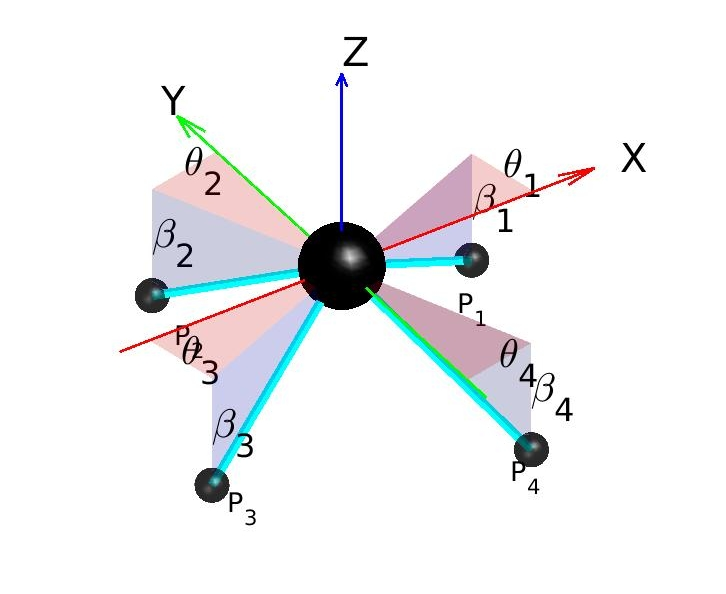
\includegraphics[width=\textwidth]{images/drone_design.jpg}
\end{minipage}
\hfill
\begin{minipage}[t]{0.3\textwidth}
  \centering
  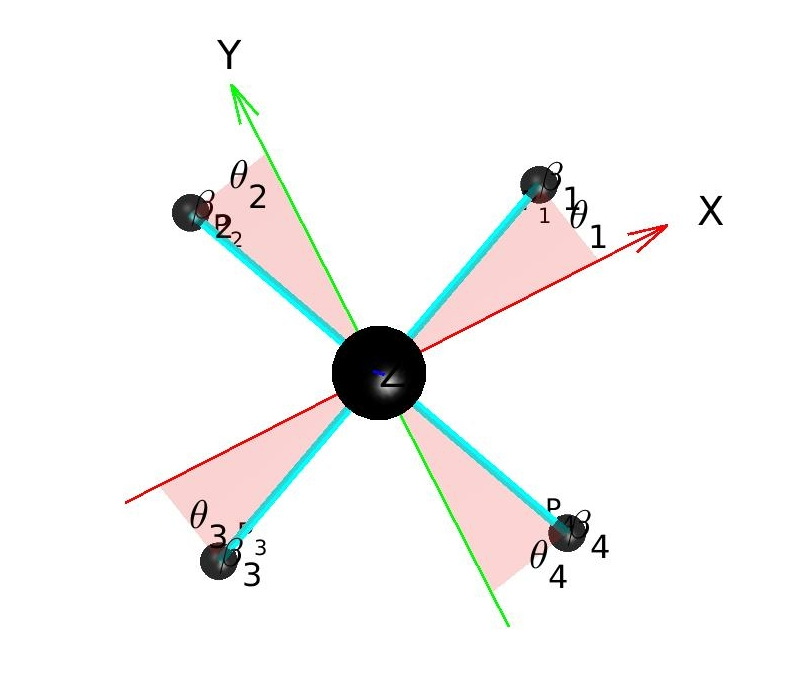
\includegraphics[width=\textwidth]{images/drone_design1.jpg}
\end{minipage}
\hfill
\begin{minipage}[t]{0.3\textwidth}
  \centering
  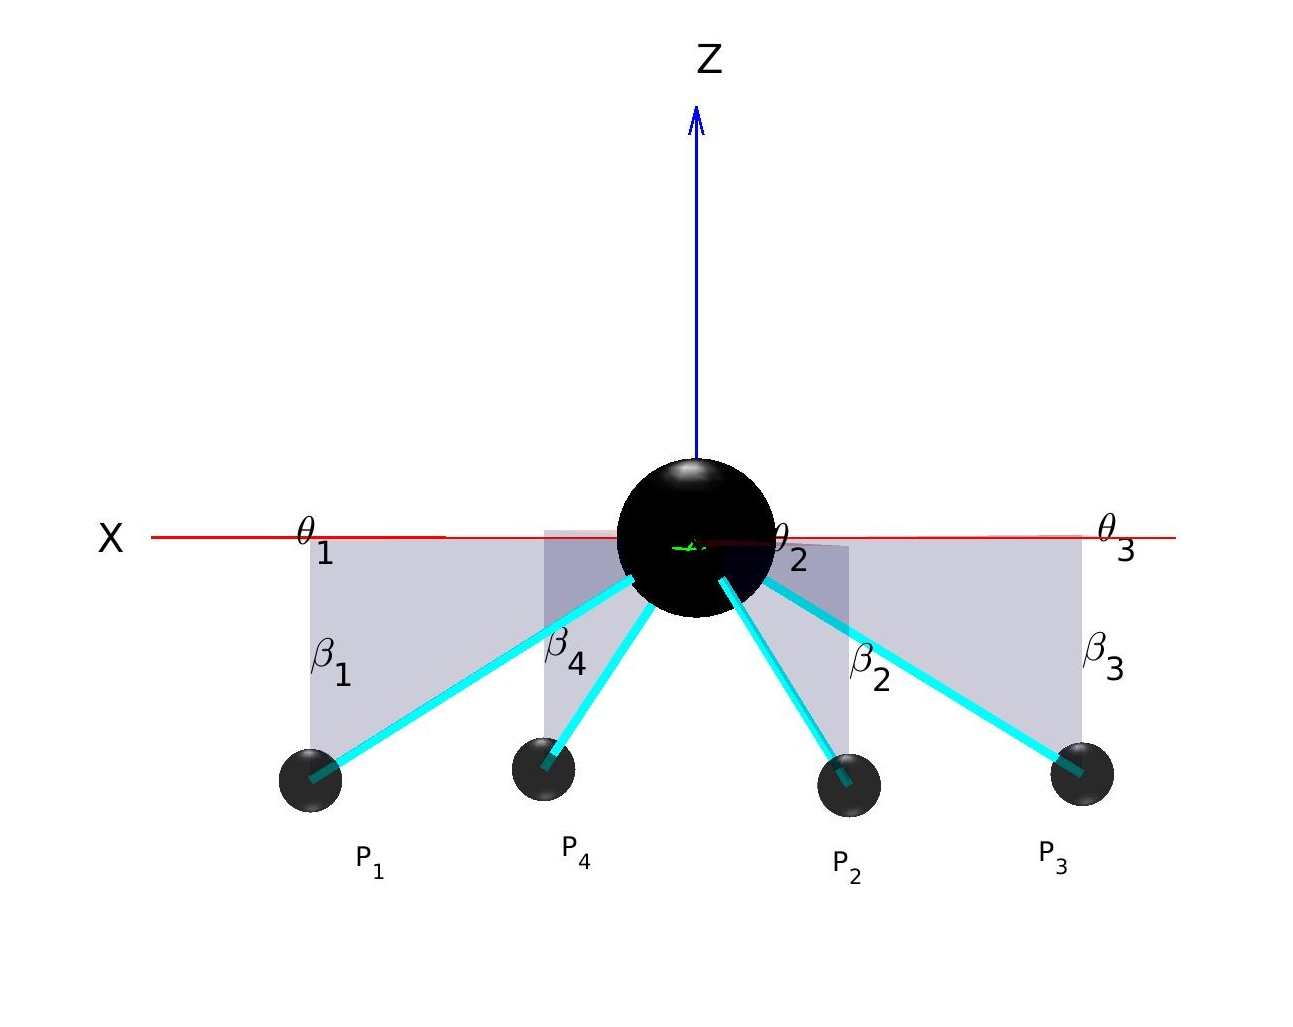
\includegraphics[width=\textwidth]{images/drone_design2.jpg}
\end{minipage}
\caption{Quadcopter to illustrate the parameters that define the morphology of an
MAV ($n = 4$, $\beta = [30, 30, 30, 30] [^{\circ}]$, $\theta = [22, 22, 22, 22]
[^{\circ}]$, and $L = 0.4 [m]$).}
\label{fig:drone_design}
\end{figure}

To solve the problem an optimization engine is develope<<<<<<<<d with
Matlab$^\textrm{\textregistered}$. This tool returns the aforementioned
parameters along with other information on the corresponding MAV design.
The interesting drone designs outpeutted by the tool are then simulated on
Gazebo\footnote{An open source robot simulator \citep{noauthor_gazebo_nodate}.}
and the control of the different models is achieved using a Robotic Operating
System\footnote{An open source collection of software that help developers to
create robot applications \citep{rostutorials}.} (ROS) node.\\
This chapter first covers the theory needed to obtain a generalize mathematical
model for a n-rotor MAV with an arbitrary morphology. Then, the optimization
problem is defined. Afterwards, the optimization tool is described. In the end,
the theoretical background needed to perform the simulations is covered.

\section{Modelisation of MAVs}
\label{sec:modeling_mav}
The following dynamical model for an n-rotor MAV is greatly inspired from the
model in \citep{ryll_modeling_2012}.
\subsubsection{Assumptions}
\label{sec:assumptions}
\subsubsection{Equations of motion}
\label{sec:equations}
\subsubsection{}
\label{sec:assumptions}

\begin{figure}[h]
  \centering
  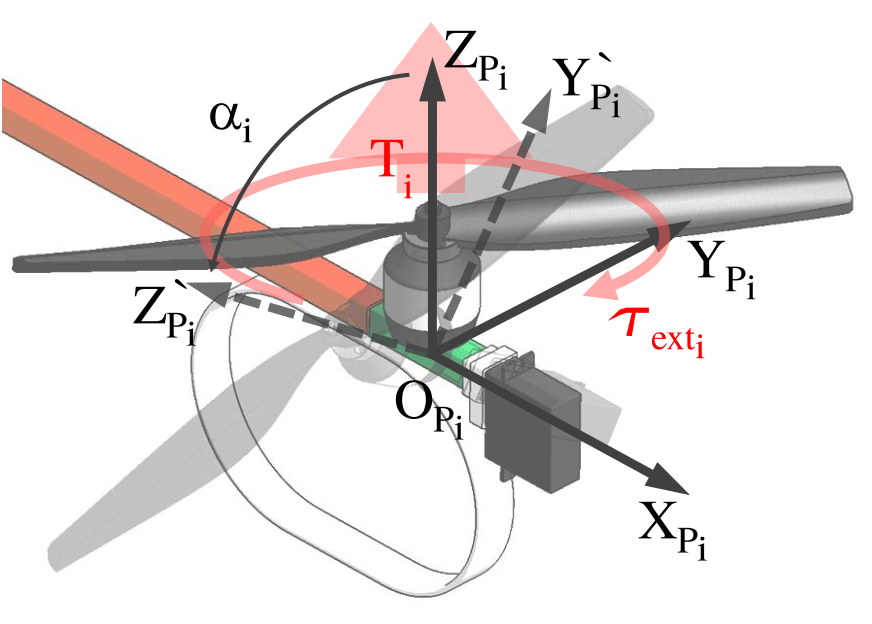
\includegraphics[width=0.3\textwidth]{images/tilt_model.png}
  \caption{Representation of the i-th tilting arm \citep{ryll_modeling_2012}.}
  \label{fig:hexacopter}
\end{figure}

\section{Optimization problem}
\label{sec:optimization_problem}
Define morphology optimization problem

\section{Optimization tool}
\label{sec:optimization_tool}
Show resulting optimization tool.

\section{Simulation Approach}
\label{sec:control_approach}
